\documentclass[a4paper,10pt]{article}
\usepackage{hyperref}
\usepackage{graphicx}
\usepackage{url}

% Title Page
\title{Convolutional Neural Networks}
\author{Faur Anca Maria}


\begin{document}
\maketitle



\tableofcontents
\section{Overview}


\quad This assignment aims to exemplify the use of the machine learning Tensorflow Framework in order to build a convolutional network classifier. The Keras high-level neural-network API used in order to enable fast experimentation.     

\vspace{5mm} %5mm vertical space

The official websites proving information about tensorflow and keras are:
\begin{itemize}
\item \url{https://www.tensorflow.org/}
\item \url{https://keras.io/}
\end{itemize}

\subsection{Running instructions}
	\subsubsection{Install instructions}
     \begin{enumerate}
 		\item I downloaded Python 3.6 version and introduced Python as enviromental variable
		\vspace{5mm} %5mm vertical space
	
	 	\item I downloaded the Anaconda installer and introduced Anaconda as enviromental variable
	
		\vspace{5mm} %5mm vertical space
		\item I created a tensorflow enviromental
	
		\texttt{conda create -n tensorflow pip python=3.5} 
		\vspace{5mm} %5mm vertical space
	
		\item I activated the tensorflow enviromental
	
		\texttt{C:> activate tensorflow}
		\vspace{5mm} %5mm vertical space
	
		\item I followed the requirements for installing the GPU support from the official tensorflow website
		\begin{itemize}
		 \item CUDA® Toolkit 9.0. .
		 \item The NVIDIA drivers associated with CUDA Toolkit 9.0.
		 \item cuDNN v7.0. 
		\end{itemize}
		
		
		\vspace{5mm} %5mm vertical space
		
		\item I installed the GPU tensorflow version using
	
		\texttt{
		(tensorflow) pip3 install --upgrade tensorflow-gpu}
		
		\end{enumerate}
	 	
		\subsubsection{Running example}
			For checking the installation, I run the following example:
		 \begin{enumerate}
		\item I cloned a repository containing a tensorflow pre-made estimator
		
		\texttt{git clone https://github.com/tensorflow/models}
		\vspace{5mm} %5mm vertical space
		
		\item I tested the pre-made estimator on the Iris dataset
		
		\texttt{cd models/samples/core/get\_started/ python premade\_estimator.py}
		\vspace{5mm} %5mm vertical space
		
		\item I obtained the accuracy of predicting each class (Setosa, Versicolor, Virginica) 
		 \end{enumerate}
	
 \subsection{Introduction to Neural Network}
 
  \subsubsection{Biological and Artificial Neuron}
  \quad Our nervous system consists of about 100 billion interlinked neurons that are capable of carrying out complex computations. Each neuron has an antenna zone comprising the cell body and extremities, one axon and thousands of dendrites. Sufficient electrical activity on a neuron’s dendrites causes an electrical pulse to be sent down the axon, where it may activate other neurons.  
    %5mm vertical space
   \begin{figure}[!htbp]
   	\centering
   	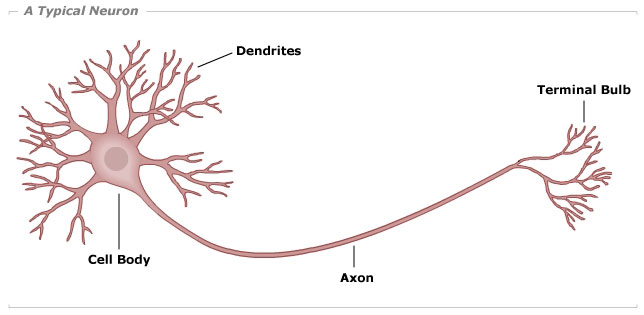
\includegraphics[width=0.5\textwidth]{neuron.jpg}
   	\caption{Biological neuron}
   \end{figure}

   
 \quad An artificial neuron is a mathematical function conceived as a model of biological neurons and represents the elementary unit in an artificial neural network. The artificial neuron receives one or more inputs (as through the neural dendrites) and computes a weighted sum to produce an output (as the action potential which is transmitted along the axon). 
   
   $$ \sum_{i \in [0,n]} = weight_{i} * x_{i}  $$
   
   The weighted sum is passed through an activation/transfer function.
   
   \begin{figure}[!htbp]
   	\centering
   	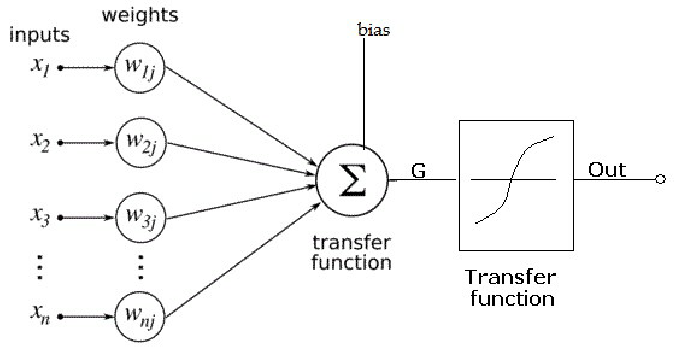
\includegraphics[width=0.5\textwidth]{artif.png}
   	\caption{Artificial neuron}
   \end{figure}
  	\vspace{5mm} %5mm vertical space
  	
  \subsubsection{Activation Functions}
  \quad An activation function is used in order to introduce non-linear properties into the network. It takes the weighted sum of the inputs, adds direction and decides whether to activate a particular artificial neuron or not.
  \begin{itemize}
  	\item \texttt{Signoid function}
  	
  	 \quad The sigmoid function or Logistic function is an activation function where it scales the values between 0 and 1 by applying a threshold. 
  	 $$ f (x) =  \frac{\mathrm{1} }{\mathrm{1} + e^{-x} }  $$ 
  	 \quad The figure below indicates the shape of the function. 
  	\begin{figure}[!htbp]
  		\centering
  		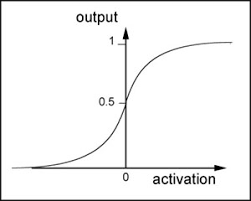
\includegraphics[width=0.5\textwidth]{sigmoid.png}
  		\caption{Sigmoid function}
  	\end{figure}
  \vspace{5mm} %5mm vertical space
  
  	\vspace{5mm} %5mm vertical space
 	\item \texttt{ReLU function}
 	
 	\quad ReLU(Rectified Linear Unit)  is one of the most widely used activation function. The benefits of ReLU is the sparsity, it allows only values which are positive and negative values are not passed which will speed up the process. 
 	$$ f (x) =  max(0,x)  $$ 
 	\quad The figure below indicates the shape of the function. 
 	\begin{figure}[!htbp]
 		\centering
 		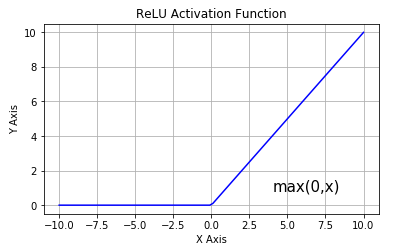
\includegraphics[width=0.5\textwidth]{relu.png}
 		\caption{ReLU function}
 	\end{figure}
 	
 	
 	
 	\vspace{5mm} %5mm vertical space
 	\item \texttt{Softmax function}
 	
 	\quad The softmax function is especially used when multi-class classification is desired. It squashes the outputs of each neuron to be between 0 and 1, just like a sigmoid function, but it also divides each output such that the total sum of the outputs is equal to 1.
 	
 	\quad The output of the softmax function is equivalent to a categorical probability distribution, it tells you the probability that any of the classes are true.
	$$ f(x)_j = \frac{e^{z_{j}}}{\sum_{k=1..classes } e^{z_{k}}} $$
	\end{itemize}

\subsubsection{Neural Network Topology}

\quad Neural networks are composed of layers of neurons. 
They receive an input (a single vector) through the input layer, and transform it through a series of hidden layers. Each hidden layer is made up of a set of neurons, where each neuron is fully connected to all neurons in the previous layer, and where neurons in a single layer function completely independently and do not share any connections. The last fully-connected layer is called the output layer and in classification settings it represents the class scores.


\begin{figure}[!htbp]
	\centering
	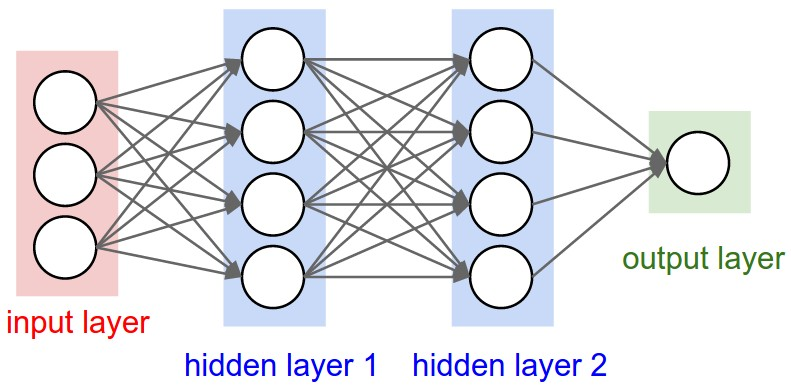
\includegraphics[width=0.5\textwidth]{layers.jpg}
	\caption{Neural Network Layers}
\end{figure}

\quad The activation functions of the neurons depend upon their position in the layered structure.
\begin{itemize}
	\item for the hidden layers, we might use the Sigmoid or ReLU activation functions
	\item for the output layer, if our model is a classifier, we would use Sigmoid activation function for binary classification and Softmax activation function for multi-class classification  
\end{itemize}

\quad Neural Networks don't scale well for images due to the high number of parameters (weights) that must be learned. For example, an image of more respectable size, e.g. 200x200x3, would lead to neurons that have 200*200*3 = 120,000 weights. Clearly, this full connectivity is wasteful and the huge number of parameters would quickly lead to overfitting.

\vspace{5mm} %5mm vertical space

 \subsection{Backpropagation Algorithm}
 
 \quad Backpropagation is a method used in artificial neural networks for the calculation of the weights for the inputs and connections between neurons. In the context of learning, backpropagation adjusts the weight of neurons by calculating the gradient of the loss function. This technique is also sometimes called backward propagation of errors, because the error is calculated at the output and distributed back through the network layers.
 
 \quad Let's consider  Mean-Squared-Error is used for the loss function in order to compute the error of the model.
  $$ J(X) = \frac{1}{m} * \sum_{i \in [1,m]}  {(y_{i} - yPredicted_ {i}})^2  $$
  
  where 
  
  \quad J = loss function 
  
  \quad X = set of examples  $x_{i}$ i=1..m
  
  \quad m = no of examples in set X
  
  \quad $y_{i}$ = the actual class of example $x_{i}$ 
  
  \quad $yPredicted_{i}$ = the predicted class of example $x_{i}$
  
 
 \begin{enumerate}
 	\item \texttt{Random initialization:} initialize all weights randomly
 	\item \texttt{Forward propagation:} make predictions for all the training examples, layer by layer from layer 1 to layer L. 
 	\begin{itemize}
 		\item Calculate the inputs to the units in that layer (weighted sums)
 		\item Calculate the outputs of the units in that layer (using activation function)
 	\end{itemize}
 
	\item \texttt{Backward propagation:} calculate the error signals at layer by layer in reverse, from layer L to layer 1.
		\begin{itemize}
		\item Calculate the error signals for the units in that layer
		
		\quad \quad Consider the connection between a neuron of layer Lp connected to a neuron of layer Lp-1
		
		\quad The error of the neuron of layer Lp is the multiplication between the activation function of the neuron of layer Lp-1 and the error signal of the neuron Lp-1 (formula for the error signal is too complicated for the purpose of this introduction)
		
		\quad This relation shows that the errors on one layer are based on the error signals of subsequent layers. 
		  
		\item Update all the weights according to the gradient of the loss of previous layer. 
		
		\quad The update is also influenced by a learning rate parameter which varies between 0 and 1. If this parameter is close to 0, the update of weights occurs slowly and more steps are required for the model to converge, but if the learning rate is too close to 1, the update is too drastic and the model may skip the optimal solution or even diverge. 
		 $$ newWeight = oldWeight - \alpha *\frac{\partial J}{\partial w} $$
		 where $\alpha$ = learning rate parameter
		
		\end{itemize}
  \end{enumerate}
 
 \vspace{5mm} %5mm vertical space
 
 
 \subsection{Introduction to Convolutional Network}
 
 \quad Convolutional Neural Networks (convnets) are very similar to ordinary Neural Networks as both are made of layers of neurons that have learnable weights. However, they have a more sensible approach regarding the neurons connections. Convolutional Networks are widely used in computer vision and in other perceptual problems including speech recognition and natural language processing.  
 \subsubsection{Hierarchical approach }
 
 \quad Convolutional Networks model the primate vision system where there is a hierarchy of neurons within the visual cortex.
 \begin{itemize}
 	
 \item In the lowest layers,
 neurons have small local receptive fields and respond to stimuli in a limited region of the visual field (e.g. spots of light)
 
 \item In higher layers,
 they combine the outputs of neurons in the lower layers and are able to respond to more complex stimuli (e.g. lines at particular orientations)
 
 \item In the highest layers,
 they respond to ever more complex combinations, such as shapes and objects
  \end{itemize}

	
	\quad As a result, the convolutional networks are able to learn features that are translation invariant (e.g. the cat can be recognized no matter its position in the image)

 \subsubsection{Layer Types}
 	\begin{itemize}
 		\item Dense Layers
 		
 		\quad Dense layers or fully connected layers connect every neuron in one layer to every neuron in another layer.
 		\vspace{5mm} %5mm vertical space
 		
 		\item Convolutional Layers
 		
 		\quad A convolutional layer is a 3D tensor of neurons, whose shape is (height, width, depth). The depth represents the number of feature maps, each feature map in a layer is responsible for learning a certain feature. Within one feature map, all neurons share the same weights resulting in the translation invariance of the learned features. 
 		
 		
 		\quad In a convolutional layer, every neuron in that layer has connections from only a small rectangular window of neurons in the preceding layer, typically  3x3 or 5x5.
 		
 		 \begin{figure}[!htbp]
 		 	\centering
 		 	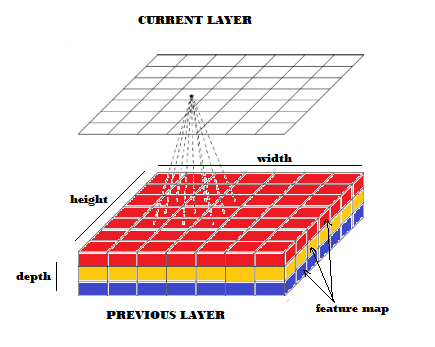
\includegraphics[width=0.5\textwidth]{convnet.png}
 		 	\caption{Convolutional Layer}
 		 \end{figure}
 		
 		\vspace{5mm} %5mm vertical space
 		\item Pooling layers
 		
 		\quad Pooling layers are used to shrinks the number of neurons in higher layers in order to:
 		\begin{itemize}
 			\item reduce the amount of computation
 			\item reduce the number of parameters to be learned
 			\item create a hierarchy in which higher convolutional layers contain information about the totality of the
 			original input features
 		\end{itemize}
 	
 		\quad The pooling layers work on rectangular windows: neurons in the pooling layer are connected to windows of neurons in the
 		previous layer. 
 		
 	 	\quad MaxPooling is a particular type of pooling layer where a neuron receives the outputs of the neurons in the window in the previous layer and outputs only the largest of them.  
 		
 		
 		\begin{figure}[!htbp]
 			\centering
 			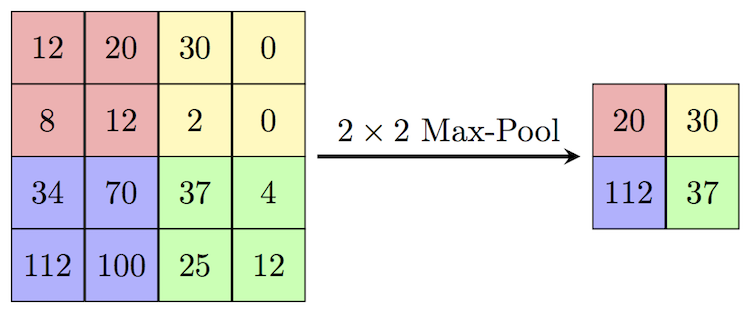
\includegraphics[width=0.5\textwidth]{maxpool.png}
 			\caption{Max Pooling Layer}
 		\end{figure}
 
 	\end{itemize}
 	\vspace{5mm} %5mm vertical space
 
 \subsubsection{Convolutional Network Topology}
 
 \quad A usual convolutional network is composed of several convolutional layers separated by pooling layers, followed by a flatten layer that transforms the tensor of neurons in a 1D array and the last layers are fully connected layers. 
 
 \quad The figure below shows an example of a convolutional network that is used to classify hand-written digits. The inputs of the network are 28x28 grey-scale images and there are 10 output neurons, each one activating for a digit between 0-9. 
  
 	\begin{figure}[!htbp]
 	\centering
 	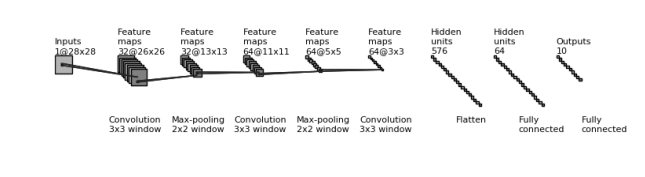
\includegraphics[width=0.5\textwidth]{convnetTopo.png}
 	\caption{example of Convolutional Network}
 \end{figure}
 
 
 \subsection{The overfitting problem}
	\subsubsection{Detecting overfitting}
	\quad Overfitting occurs when we are training a model that is too complex for the amount of the trainig data and for its noisiness. As a result, the learning algorithm fits too well the examples of the train set (including its outliers), but loses its power of generalization. When it is supposed to analyse new examples, e.g. from the validation/test sets, we notice that the loss function outputs an error that is way above the error on the train set. 
	
	\quad Overfitting can be easily spotted if we plot the error of the training and validation set. In the case of overfitting, the training error is small and  there remains a big gap between training error and validation error. 
	
	\begin{figure}[!htbp]
		\centering
		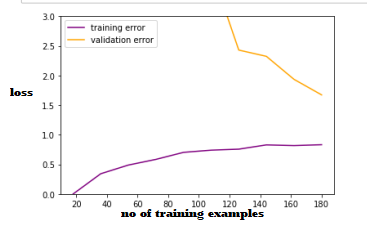
\includegraphics[width=0.5\textwidth]{overfit.png}
		\caption{example of overfitting }
	\end{figure}

	\quad The figure also analyses how the number of training examples influences the learning, we notice that, until a certain point, the increase of the number of examples improves the quality of the model.  
	

	\quad A model that is suitable for its training examples would have a plot as the one below. We can see that as the number of examples learned increases, the error decreases. Moreover, the gap between the train error and the validation error narrows and they converge. 
	
		\begin{figure}[!htbp]
		\centering
		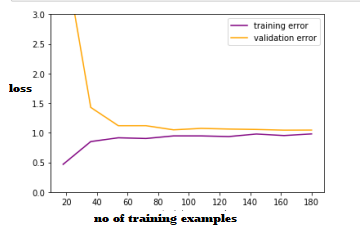
\includegraphics[width=0.5\textwidth]{suitable.png}
		\caption{example of a suitable model}
	\end{figure}
 	\vspace{5mm} %5mm vertical space
 
 \subsubsection{Solutions for Neural Networks}
 \begin{enumerate}
 	\item Reducing the network's size
 	
 	\quad A neural network can be simplified by reducing the number of parameters, through reducing the number of hidden layers and/or the number of neurons inside the hidden layers.
 	
 	\item Weight regularization
 	
 	\quad The complexity of the model can be reduced by reducing the range for the values of the weights parameters. Weight regularization means forcing the weights values to be small through evaluating the model using a loss function that is conditioned by the small values of the weight parameters also. 
 	\begin{itemize}
 		\item Lasso: we penalized by the l1-norm (the sum of their absolute values of the weights)
 		\item Ridge: we penalized by the l2-norm (the sum of the squares of the weights)
 		\item A hyperparameter , called the 'regularization parameter' controlled the balance between fitting the data versus shrinking the weights 
 	\end{itemize}
 	
 	\item Dropout
 	
 	\quad The complexity of the model can be reduced by altering the number of neurons during training. We give neurons a probability \texttt{p} to be dropped out in the training process.
 	
 	
 	\quad For every mini-batch in the training set:
 	\begin{itemize}	
 	\item In the forward propagation, decide which neurons will be dropped with probability  \texttt{p}.
 	Set the activations of the dropped neurons to zero
 	and divide the activations of the kept neurons by  \texttt{(1-p)} (as the kept neurons will receive inputs from more neurons)
 	\item In the backpropagation, ignore the dropped out neurons
 	\end{itemize}
 	
 \end{enumerate}

 \section{Proposed problem}
  \subsection{Specification} 
  
  \quad This assignment aims to build a classifier able to recognize between 10 different species of monkeys. The classifier is built using the Convolutional Neural Network technique. For machine learning, the Tensorflow framework is used with the help of the Keras high-level neural network API.
  
    \subsection{Data representation}
  
   \quad The dataset used consists of JPEG format images of 10 different species of mokeys. The data is divided into 2 folders, training and validation. The folders contain 10 sub-folders labelled as n0~n9, each  containing images of a different species of monkey. The total number of images is around 1400. The dataset can be found at the link:
   
   \url{https://www.kaggle.com/slothkong/10-monkey-species}
   
   \quad The images are decoded and uncompressed in grids of 150x150 RGB pixels. The values of the pixels would be too high for the model to process (given a typical learning rate), so values are scaled between 0 and 1 using 1/255 factor.
   
  
  \subsection{Implementation Overview} 
  \quad The problem of classifying the monkey species is solved using convolutional networks. The base network is composed of 4 convolutional layers (and max-pooling layers in between) and 2 fully connected layer. In order to respond to the problem of overfitting, the base network is then slightly modified resulting in the network having weight regularization and the network using dropout. The number of examples is artificially increased using data augumentation. 
  
  \quad Moreover, the assignment exemplifies the use of a pre-trained model in order to solve the monkey problem.
  
  \quad The proposed neural networks have an accuracy between 60\% to 70\%.

  \subsection{The Base Convolutional Network}
\quad \quad The following Keras segment of code presents the base convolutional network.
 
 \begin{figure}[!htbp]
 	\centering
 	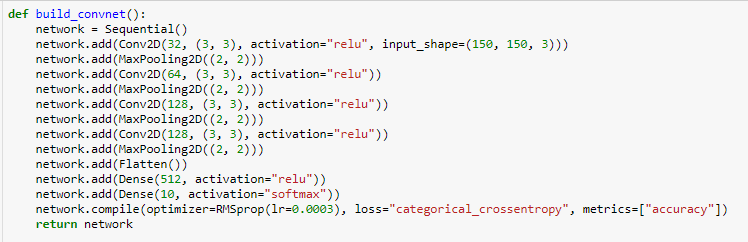
\includegraphics[width=0.5\textwidth]{base_network.png}
 	\caption{base network}
 \end{figure}
 \vspace{5mm} %5mm vertical space
 
 
  \quad Each convolutional layer has the following parameters (in order):
  \begin{itemize}
  	\item the number of feature maps
  	\item the size of the convolutional window between 2 consecutive layers
  	\item the activation function 
  \end{itemize}
 
 \quad The last two layers are fully connected (dense), the first parameter represents the number of neurons and the second one represents the activation function. In order to classify between 10 classes, the last layer contains 10 neurons and softmax function is used in order to obtain a probability distribution between the classes. The class predicted with the highest probability is the predicted class. 
 
 \quad In order to optimize the predictions, I have chosen the RMSprop variant of gradient descent for backpropagation calculus. The learning rate has been set to 0.0003.
 \vspace{5mm} %5mm vertical space
 
 \quad The structure of the network can be better understood from the following summary.
 
  \begin{figure}[!htbp]
 	\centering
 	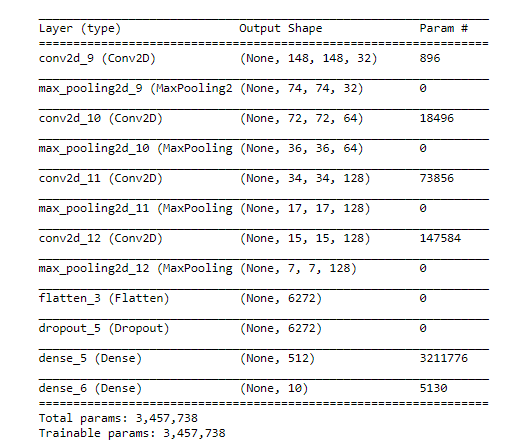
\includegraphics[width=0.5\textwidth]{network_summary.png}
 	\caption{Network Summary}
 \end{figure}
 \vspace{5mm} %5mm vertical space
 
 \quad The learning process hyperparameters have been set to:
  \begin{itemize}
 	\item number of epochs = 30 (epoch = pass over the all training examples)
 	\item number of steps\_per\_epoch = 57 (in order to cover all 1097 training examples in 20 epochs)
 	\item number of validation\_steps=13 (in order to cover all 272 validation examples in 20 epochs)
 	\item the batch size = 20 (the batch size = no of examples propagated through the network at once. A smaller number saves memory and improves speed due to simpler backpropagation updates on weights. However, the updates of the weights can be misleading as they are influenced by the prediction over a small partition of the dataset, not on the entire dataset).
 	\item early\_stopping = 2 (in order to speed up the learning process, the model stops training when the loss function has stopped improving for more than 2
 	epochs ) 
 		
 \end{itemize}

\quad The initial prediction has an accuracy of approximately 69\%. The following image shows the evolution of the loss function and accuracy metric during the first epochs until the process has been interrupted due to early stopping.
 
 \begin{figure}[!htbp]
	\centering
	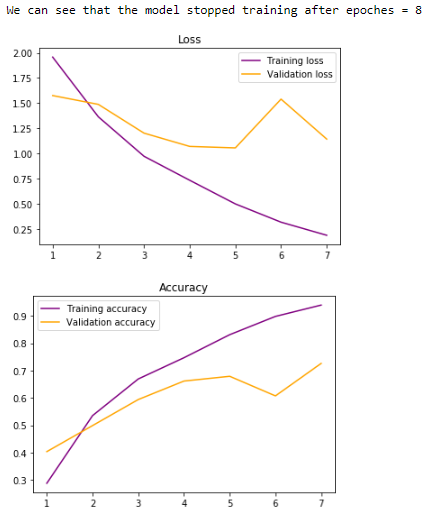
\includegraphics[width=0.5\textwidth]{lossacc.png}
	\caption{Loss and Accuracy evolution in epochs}
\end{figure}
\vspace{5mm} %5mm vertical space
  
\quad In the last epoch, we notice that there still is a big gap between the training and the validation examples. That gap suggests the problem of overfitting. 

  \subsection{Strategies against Overfitting}
  \subsubsection{Data Augmentation}
  
  \quad \quad Data augmentation is another way we can reduce overfitting on models, where we increase the amount of training data using information only in our training data. However the obtained examples are not as good as new examples. 
  
  \quad In order to obtain more examples, I used image transformations on the training images. 
  
   \begin{figure}[!htbp]
  	\centering
  	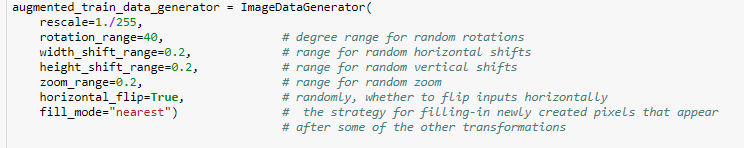
\includegraphics[width=0.5\textwidth]{augment.png}
  	\caption{Image transformations used for data augmentation}
  \end{figure}
  \vspace{5mm} %5mm vertical space
  
   \begin{figure}[!htbp]
  	\centering
  	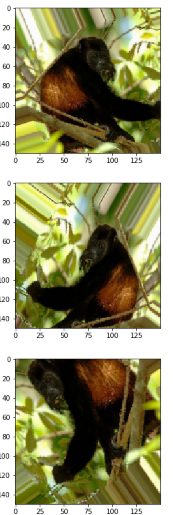
\includegraphics[width=0.5\textwidth]{augmentimg.png}
  	\caption{Images obtained due to data augmentation}
  \end{figure}
  \vspace{5mm} %5mm vertical space
  
  \subsubsection{Weight Regulation}
  \quad For weight regularization, the convolutional network uses Ridge l2-norm. 
  
  \begin{figure}[!htbp]
  	\centering
  	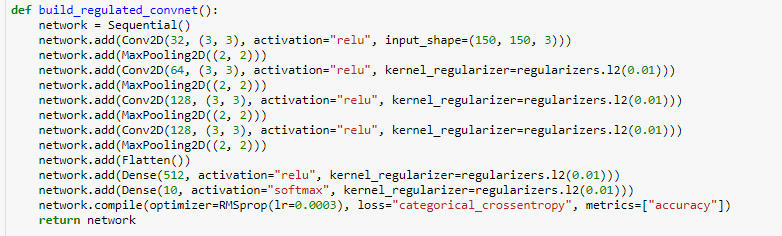
\includegraphics[width=0.5\textwidth]{regulated.png}
  	\caption{Convolutional Network with weight regularization}
  \end{figure}
  \vspace{5mm} %5mm vertical space
  
   \subsubsection{Dropout}
   \quad Dropout is usually used in the dense layers as the number of parameters of the convolutional layers isn't considered big enough to result in overfitting. 
   
     \begin{figure}[!htbp]
   	\centering
   	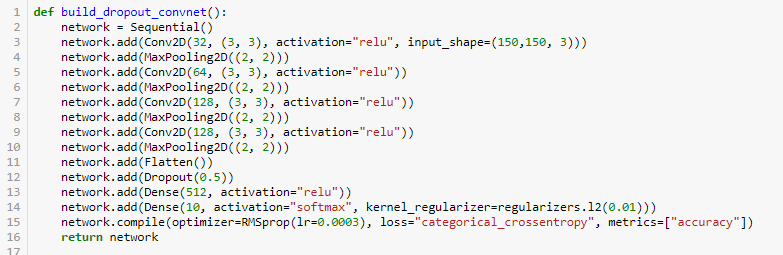
\includegraphics[width=0.5\textwidth]{dropout.png}
   	\caption{Convolutional Network with dropout}
   \end{figure}
   \vspace{5mm} %5mm vertical space
   
   \quad Even if the classification accuracy doesn't improve, from the following images we can notice that the gap between the training examples and the validation examples loss and accuracy was reduced.
     
     \begin{figure}[!htbp]
   	\centering
   	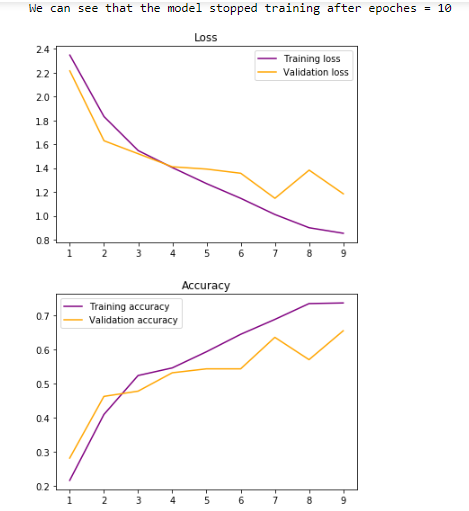
\includegraphics[width=0.5\textwidth]{lossaccdropout.png}
   	\caption{Loss and accuracy evolution in epochs when using dropout}
   \end{figure}
   \vspace{5mm} %5mm vertical space
   
   
   \subsection{Transfer Learning}
   \quad \quad Transfer learning is a machine learning method where a model developed for a task is reused as the starting point for a model on a second task.
   
   \quad Image classifying networks, especially if they contain few examples in the training set, can use pre-trained models. The pre-trained models have been trained on large datasets such as the ImageNet 1000-classes images (which recognize 1000 different objects). 
   
   \quad The use of pre-trained models makes sense due to the hierarchical approach of convolutional networks. If the trained model is very good at recognizing animals we can use its layers in order to detect features that interest us in the monkey classification problem as fur type, eye shape and so on. The trick consists in modifying the last layer of the pre-trained model in order to match our classification problem (to have 10 neurons,one for each monkey species). The update of the weights is done only on the connection between the last layer of the pre-trained model and the added last layer (fully connected layers).
   
   \quad Moreover, for obtaining great results, it is important that the pre-trained model had used images similar to the images of the new classifier. For example, a pre-trained model on medical tomography images would result in a low-performance classifier for images from outer space.
   
   \quad I have used the ResNet50 pre-trained model and the resulting classification accuracy is around 60\%.
  
   \quad A furthermore improvement would be fine-tuning the model which means allowing the weight updates also on the last layers of the pre-trained model. The first layers can be "frozen" as they are good at detecting the simple shapes.     
\section{Conclusion}

\quad This assignment aimed to classify 10 species of monkeys. The accuracy of the obtained model is between 60\% and 70\%, I think this a good score considering the similarities of the monkeys and the reduced size of the training dataset. Moreover, this assignment gives an introduction to deep learning and explains different strategies for improving image classification.

\section{Biography}
 \begin{enumerate}
	\item biological neuron
	
	\url{http://neurosciencenews.com/neurons-synapses-neuroscience-5119/}
	\url{https://online.science.psu.edu/bisc004_activewd001/node/1907}
	
	\item artificial neuron
	
	\url{https://en.wikipedia.org/wiki/Artificial_neuron}
	
	\item activation functions
	
	\url{https://analyticsindiamag.com/most-common-activation-functions-in-neural-networks-and-rationale-behind-it/}
	\url{https://github.com/Kulbear/deep-learning-nano-foundation/wiki/ReLU-and-Softmax-Activation-Functions}
	
	\item topology of layers
	 
	\url{https://www.pyimagesearch.com/2016/09/26/a-simple-neural-network-with-python-and-keras/}
	
	\item neural network
	
	\url{http://www.cs.ucc.ie/~dgb/courses/ai2/08_neural_networks.pdf}
	
	
	\item convolutional network
	
	\url{https://en.wikipedia.org/wiki/Convolutional_neural_network}
	\url{http://www.cs.ucc.ie/~dgb/courses/ai2/13_convnets.pdf}
	
	\item conv2D
	
	\url{https://www.tensorflow.org/api_docs/python/tf/nn/conv2d}
	
	\item backpropagation
	
	\url{http://www.cs.ucc.ie/~dgb/courses/ai2/10_backprop.pdf}
		
	\item overfitting
	
	\url{http://www.cs.ucc.ie/~dgb/courses/ai2/05_over_n_under_fitting.pdf}
	\url{http://www.cs.ucc.ie/~dgb/courses/ai2/12_nn_overfitting.pdf}
	\url{https://chatbotslife.com/regularization-in-deep-learning-f649a45d6e0}
	\url{https://blog.keras.io/building-powerful-image-classification-models-using-very-little-data.html}
		
	\item transfer learning
	
	\url{https://www.pyimagesearch.com/2017/03/20/imagenet-vggnet-resnet-inception-xception-keras/}
	\url{https://flyyufelix.github.io/2016/10/08/fine-tuning-in-keras-part2.html}
		
	\item data augmentation
	
	\url{http://cs231n.stanford.edu/reports/2017/pdfs/300.pdf}
		
	\end{enumerate}

\end{document}          
